%--------------------------------------------------------------------------------------------------
\section{Interpretability}
\label{rel:sec_int}
As deep learning based models for Computer Vision have continued to improve in their recognition 
properties, their structure and functioning have become more opaque; in turn making these 
technologies seen as black boxes. A black-box model is defined as a model for which its 
interpretation is not straightforward for humans \autocite{petch2022opening}. In recent years 
with the assimilation of deep learning into everyday tasks, and the implicit effect these models 
are having on human lives; the novel research field of \emph{Interpretability} has been brought 
forth to open up this black-box behaviour. Different scholars have approached intepretability 
alongside different directions. Starting with the work of \cite{li2018deep}, interpretability is 
suggested to present two categories, \emph{Transparency} and \emph{Post-hoc Interpretability}.
For the former, Lipton argues that it follows modifications of the model or the training process, 
in order to explain the inner-workings of the model. Conversely, for the latter Lipton builds upon 
the black-box behaviour of the model, providing explanations istead based on inputs nad outputs; 
without adding any further modifications for the model or altering its training process.\\

Complementary to Lipton's proposal, \cite{guidotti2018survey} points that interpretability is 
contained along different dimensions. On one hand, a model can be understood on its entirety 
following \emph{Global} interpretation; whereas in situations where only the reasons leading to a 
specific prediction a \emph{Local} interpretation is found. Guidotti also considers time,
more specifically \emph{Time Limitation} as its availability is strictly correlated to the scenario 
where the model is used. Finally, the \emph{Nature of User Expertise} covers the last dimension of 
interpretability; where knowing the experience of an user in a given task is considered to be a 
key aspect describing the interpretability of a model.\\

In recent years \cite{zhang2021survey} suggested that three different dimensions encompass this 
study. The first dimension answers to the nature of an approach; where it can be either 
\emph{Passive} or \emph{Active}. The first direction in this dimension correlates to Lipton's 
\emph{Post-hoc interpretabity}, the latter follows the aforementioned \emph{Transparency} property.
Zhang's second dimension is addressed towards the type of explanations, where the order of 
explanatory power follows examples, into attributions, leading into hidden semantics and 
finishing in rules. The last dimension that Zhang covers explanations in the input space, 
where a \emph{Local} explanation describes the network's prediction following individual 
samples; while on another hand, a \emph{Global} explanation describes the network as a whole. This 
last dimension is similar to the first point described by \cite{guidotti2018survey}.\\

\noindent In this thesis we study interpretability following Lipton's properties towards describing 
an interpretable model, in the following subsections we go into detail in works alongside each 
property.


\subsection{Transparency}
\label{rel:sub_transp}
According to Lipton, Transparency is the opposite of the black-box behaviour of a model, therefore 
a transparent model ought to provide a sense of understanding on its innerworkings. 
%Transparency in interpretability research represents a pivotal pursuit within the broader 
%landscape of artificial intelligence. In the ever-evolving field of machine learning, 
%particularly deep neural networks, the inherent complexity of models often gives rise to a lack of 
%transparency, making it challenging to comprehend the decision-making processes. Researchers 
%focusing on transparency in interpretability seek to address this opacity by developing 
%methodologies and frameworks that not only reveal how models arrive at specific outcomes but 
%also provide a comprehensive understanding of the underlying mechanisms. The ultimate goal is to 
%empower users, stakeholders, and policymakers with the knowledge necessary to trust, validate, and 
%navigate the applications of artificial intelligence effectively. This emphasis on transparency not 
%only enhances the accountability of AI systems but also contributes to broader societal acceptance 
%and ethical deployment of these powerful technologies.
Approaches are grouped in a number of categories according to the type of the given explanation. \\

\noindent \emph{Rule-based methods} (\cite{wu2018beyond}, \cite{wu2020regional}) train a decision tree as a 
surrogate regularization term to force a network to be easily approximated by a decision tree.\\

\noindent \emph{Hidden semantics-based methods} (\cite{bau2017network}, \cite{zhou2018interpreting}, 
\cite{zhang2018interpretable}, \cite{zhou2014object},\cite{bohle2022b}. \cite{bohle2024b}) aim to 
make a convolutional network learn disentangled hidden semantics with hierarchical structure or 
object-level concepts.\\

\noindent \emph{Prototype-based methods} (\cite{li2018deep}, \cite{chen2019looks}) learn a set of prototypes 
or parts as an intermediate representation in the network, which can be aligned with categories.\\

\noindent \emph{Attribution-based methods} (\cite{ismail2021improving}, \cite{Zhou_2022_BMVC}, 
\cite{ross2017right}, \cite{ghaeini2019saliency}) usually modify the architecture of a network or 
the training process to help post-hoc methods produce better saliency maps. Unlike 
(\cite{ross2017right}, \cite{ghaeini2019saliency}), saliency guided localization 
\autocite{Zhou_2022_BMVC} does not need ground truth explanations but replaces them with 
information bottleneck attribution \autocite{schulz2020restricting}. Finally, saliency-guided 
training \autocite{ismail2021improving} minimizes the KL divergence between the output of original 
and masked images. \\



\subsection{Post-Hoc Interpretability}
\label{rel:sub_post}

Approaches can be grouped into a number of possibly overlapping categories. 
\noindent \emph{Gradient-based methods} (\cite{adebayo2018local}, \cite{guidedbackprop}, 
\cite{baehrens2010explain}, \cite{simonyan2013deep}, \cite{smilkov2017smoothgrad}, 
\cite{bach2015pixel}, \cite{sundararajan2017axiomatic}) use the gradient of a target class 
score with respect to the input to compute the contribution of different input regions to the 
prediction. \\

\noindent \emph{\gls{cam}-based methods} (\cite{wang2020score}, \cite{chattopadhay2018grad}, 
\cite{selvaraju2017grad}, \cite{axiombased}, \cite{jiang2021layercam}, \cite{ablationcam}) 
compute saliency maps as a linear combination of feature maps, with different definitions for 
the weights.\\

\noindent \emph{learning-based methods} (\cite{chang2018explaining}, \cite{dabkowski2017real}, 
\cite{phang2020investigating}, \cite{zolna2020classifier}, \cite{schulz2020restricting}) learn an 
additional network or branch on extra data to produce an explanation map for a given input. 

\noindent \emph{Occlusion or masking-based methods} (\cite{petsiuk2018rise}, 
\cite{fong2017interpretable}, \cite{fong2019understanding}, \cite{schulz2020restricting}, 
\cite{ribeiro2016should}) apply a 	number of candidate masks in the input space, measure their 
effect on the prediction and then combine them into a saliency map. Masking in feature space 
has been explored too \autocite{schulz2020restricting}. 


%--------------------------------------------------------------------------------------------------
\paragraph{CAM-based saliency maps}
In this thesis we take particular interest in proposing and evaluating our interpretability 
methodologies based on \gls{cam}. In particular, we find CAM to be an appealing approach because of 
its ease of use and adaptation to interpret existing models. Moreover, it can be argued that while 
it is possible find and use a plethora of the most popular models towards recognition; providing 
explanations ought to be similarly easy to use, a property that CAM-based models share.

One property that \glspl{cnn} display is the presence of semantic information found within the 
deepest layers prior to the classifier. In detail, it has been observed that these kind of models 
operate in a similar manner to the visual cortex in the brain; basic textures and their orientation 
is processed in shallow layers, whereas deep layers associate this information into concepts 
\autocite{hubel1959receptive}. This characteristic in turn is the main motivation behind making 
use of CAM methods: by addressing interpretations on the layers prior to the classifier, we 
reconstruct the features deemed salient according to the flow of information within a model. We 
present a representation of filter responses from texture to semantics in \autoref{fig:cnn_depth}.


\begin{figure}[t]
    \centering
    \scriptsize
    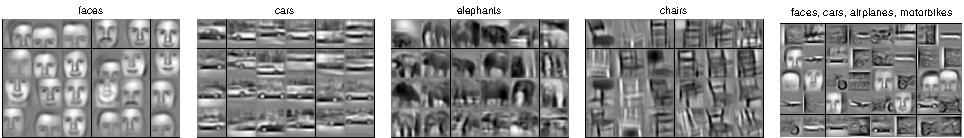
\includegraphics[width=\textwidth]{fig/rel/images/conv_layers.pdf}
    \caption{Filter response to learnt classes alongside CNN depth \autocite{lee2009convolutional}.}
    \label{fig:cnn_depth}
\end{figure}
% In particular regarding the issues addressed by \cite{bohle2021convolutional}

\paragraph{Notation}
\label{sec:oc_notation}
Consider a classifier network $:fx \cX \to \real^C$ that maps an input image $\mathbf{u} \in \cX$ to a 
logit vector $\vy = f(\mathbf{u}) \in \real^C$, where $\cX$ is the image space and $C$ is the number 
of classes. We denote by $y_c = f(\mathbf{u})_c$ the predicted logit and by $p_c = \softmax(\vy)_c 
\defn e^{y_c} / \sum_j e^{y_j}$ the predicted probability for class $c$. For layer $\ell$ 
with $K_\ell$ channels, we denote by $A^k_\ell = f^k_\ell(\mathbf{u}) \in \real^{h_\ell \times w_\ell}$ 
the feature map for channel $k \in \{1,\dots,K_\ell\}$, with spatial resolution $h_\ell \times 
w_\ell$. Because of $\relu$ non-linearities, we assume that feature maps are non-negative. 
Similarly, we denote by $S_\ell \in \real^{h_\ell \times w_\ell}$ a 2D saliency map.

\begin{figure}[t]
    \centering
        \begin{tikzpicture}[
            font={\footnotesize},
            trap/.style={trapezium, rotate=-90,trapezium angle=75},
        ]
            %% Nodes
            \node(input) at (-6, 0) {
\includegraphics[width=.1\textwidth]{fig/rel/images/cat_v2.jpg}};
            \node[above] at (input.north) {Input image $\vumod$};
            \node[draw, trap](cnn) at (-3, 0) {\rotatebox{90}{\parbox{1.0cm}{\centering{\Th{CNN}}}}};
            \node(fmaps) at (-0.5,0) {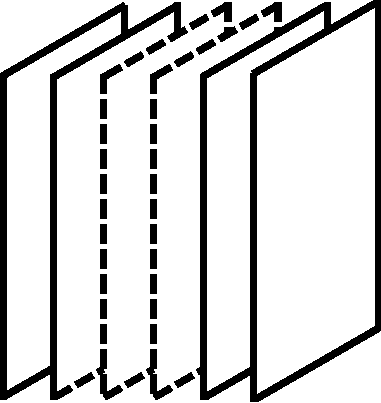
\includegraphics[width=.1\textwidth]{fig/rel/images/fmaps_side.pdf}};
            \node(fmk) at (-0.5, 1.3) {$A^k_\ell$};
            \node(classtag) at (3, 1.3) {\Th{Classifier}};
            \node(GAP) at (1.25,0.25) {$\gap$};
            \node(gapclass) at (3, 0) {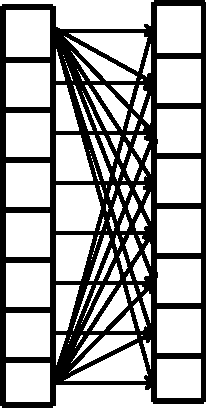
\includegraphics[width=.075\textwidth]{fig/rel/images/gapclass.pdf}};
            \node(logit) at (5, 0) {$\vy_c$};
            \node(wck) at (-0.5, -3) {
\includegraphics[width=0.02\textwidth, angle=90]{fig/rel/images/classifier.pdf}};
            \node(comb) at (-0.5, -3.5) {Weighting coefficient $w_k^c$};
            \node[draw, circle] (odot) at (-0.5, -1.8) {$\times$};
            \node(activ) at (-2.75, -1.5) {$h$};
            \node(salient) at (-3, -1.8) {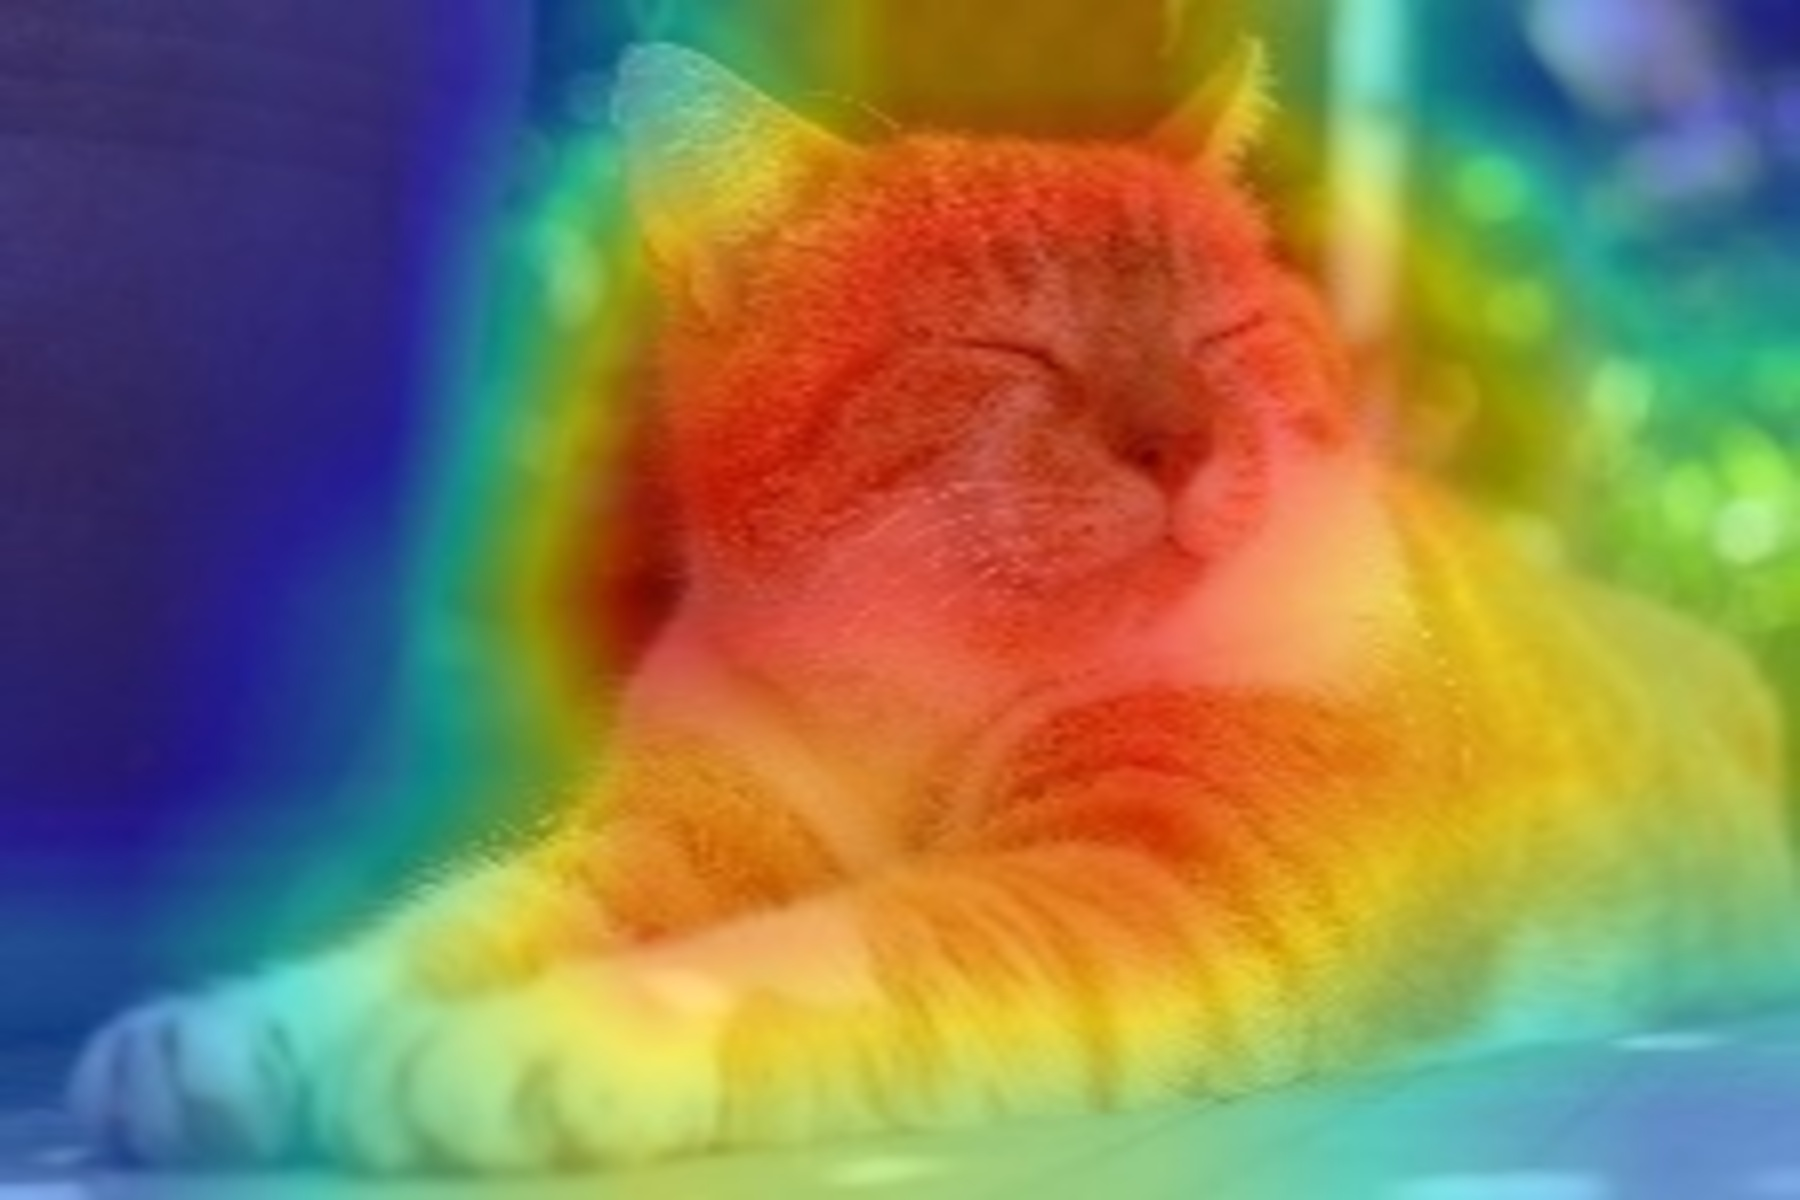
\includegraphics[width=.1\textwidth]{fig/rel/images/cat_cam.jpg}};
            \node[below] at (salient.south) {Saliency map $\mathbf{S_\ell}$};
            
            %% Edges

            \draw[->] (input.east) -- node {} (cnn);
            \draw[->] (cnn.north) -- node[above] {$\ell$} (fmaps.west);
            \draw[->] (fmaps.east) -- node {} (gapclass.west);
            \draw[->] (gapclass.east) -- node[above] {} (logit.west);
            \draw[->] (fmaps.south) -- node {} (odot.north);
            \draw[->] (wck.north) -- node {} (odot.south);
            \draw[->] (odot.west) -- node {} (salient);           

    \end{tikzpicture}
    \caption{\textbf{CAM} based methodologies overview.}
    \label{fig:cam_schema}
\end{figure}
%--------------------------------------------------------------------------------------------------


\label{sec:oc_back}

Given a layer $\ell$ and a class of interest $c$, we consider saliency maps given by the general 
formula
\begin{equation}
	S^c_\ell(\mathbf{u}) \defn h \left( \sum_k w^c_k A^k_\ell \right),
\label{eq:sal}
\end{equation}
where $w^c_k$ are weights defining a linear combination over channels and $h$ is an activation 
function. CAM \parencite{zhou2016learning} is defined for the last layer $L$ only with $h$ being the 
identity mapping and $w^c_k$ being the classifier weight connecting the $k$-th channel with 
class $c$. Grad-CAM \parencite{selvaraju2017grad} is defined for any layer $\ell$ with $h = \relu$ and 
weights
\begin{equation}
	w^c_k \defn \gap \left( \pder{y_c}{A^k_\ell} \right),
\label{eq:gcam}
\end{equation}
where $\gap$ is global average pooling.
% and $\softmax(\vy)_c = e^{y_c} / \sum_j e^{y_j}$ is the predicted probability of class $c$.
The motivation for $\relu$ is that we are only interested in features that have a positive effect 
on the class of interest, \ie pixels whose intensity should be increased in order to increase $y_c$.

Score-CAM \parencite{wang2020score} is also defined for any layer $\ell$ with $h = \relu$ and weights 
$w^c_k \defn \softmax(\mathbf{u}^c)_k$.  Softmax normalization considers positive channel contributions 
only and attends to few feature maps.
%that \alert{produce less highlighted areas in the saliency map}. \iavr{Last part unclear.}
Here, vector $\mathbf{u}^c \in \real^{K_\ell}$ measures the increase in confidence for class $c$ that 
compares a known baseline image $\mathbf{u}_b$ with the input image $\mathbf{u}$ masked according to feature 
map $A^k_\ell$, for all channels $k$:

\begin{equation}
	u^c_k \defn f(\mathbf{u} \odot n(\operatorname{up}( A^k_\ell )))_c - f(\mathbf{u}_b)_c,
\label{eq:s-cam}
\end{equation}

where $\odot$ is the Hadamard product. For this to work, the feature map $A^k_\ell$ is adapted
 to $\mathbf{u}$ first$:\operatorname{up}$ denotes upsampling to the spatial resolution of $\mathbf{u}$ and

\begin{equation}
	n(A) \defn \frac{A - \min A}{\max A - \min A}
\label{eq:norm}
\end{equation}

is a normalization of matrix $A$ into $[0,1]$. While Score-CAM does not need gradients, 
it requires as many forward passes through the network as the number of channels in the chosen layer,
 which is computationally expensive.

%--------------------------------------------------------------------------------------------------

\paragraph{Motivation}
\label{sec:motiv}

\iavr{Score-CAM considers each feature map as a mask in isolation. How about linear combinations?} 
Given a vector $\vw \in \real^{K_\ell}$ with $w_k$ its $k$-th element, let
\begin{equation}
	F(\vw) \defn f \left( \mathbf{u} \odot n \left( \operatorname{up} \left(
		\displaystyle\sum_k w_k A^k_\ell
	\right) \right) \right)_c.
\label{eq:s-obj}
\end{equation}
\ronan{If we assume that $\mathbf{u}_b = \vzero$ in~\eq{s-cam} and define $n(\vzero) \defn \vzero$ 
in~\eq{norm}, then we can rewrite the right-hand side of~\eq{s-cam} as
\begin{equation}
	\frac{F(\vw_0 + \delta \ve_k) - F(\vw_0)}{\delta},
\label{eq:s-cam2}
\end{equation}
where $\vw_0 = \vzero$, $\delta = 1$ and $\ve_k$ is the $k$-th standard basis vector of 
$\real^{K_\ell}$. This resembles the numerical approximation of the derivative $\pder{F}{w_k}(\vw_0)$,
 except that $\delta$ is not small as usual. One could compute derivatives efficiently by 
 standard backpropagation instead. It is then possible to iteratively optimize $F$ with respect
  to $\vw$, starting at any $\vw_0$.}

\iavr{As an alternative, consider masking-based methods relying on optimization in the input space, 
like \emph{meaningful perturbations} (MP) \parencite{fong2017interpretable} or 
\emph{extremal perturbations} \parencite{fong2019understanding}. In general, optimization takes the form
\begin{equation}
	S^c(\mathbf{u}) \defn \arg\max_{\vm \in \cM} f(\mathbf{u} \odot n(\operatorname{up}(\vm)))_c + \lambda R(\vm).
\label{eq:mask}
\end{equation}
Here, a mask $\vm$ is directly optimized and does not rely on feature maps, hence the saliency 
map $S^x(\mathbf{u})$ is not connected to any layer $\ell$. The mask is at the same or lower resolution 
than the input image. In the latter case, upsampling is still necessary.

In this approach, one indeed computes derivatives by backpropagation and indeed iteratively 
optimizes $\vm$. However, because $\vm$ is high-dimensional, there are constraints expressed by 
$\vm \in \cM$, \eg $\vm$ has a certain norm, and regularizers like $R(\vm)$, \eg $\vm$ is smooth in a 
certain way. This makes optimization harder or more expensive and introduces more hyperparameters 
like $\lambda$. One could simply constrain $\vm$ to lie in the linear span of $\{A_\ell^k\}_{k=1}
^{K_\ell}$ instead, like all CAM-based methods.}


